\documentclass{article}
\usepackage{../csci-246-fall2018/hw/template/fasy-hw}
\usepackage{amsmath}
\usepackage{cancel}
\usepackage{hyperref}

\author{Nathan Stouffer}
\problem{7-1}
% \problem{A-B} means Problem Set A, Problem B.
\collab{Kevin Browder}
% or give names, e.g., \collab{Alyssa P. Hacker and A. Student}

\begin{document}

\section*{Section 8.5, Problem 14}

Prove $\forall a,b \in \mathbb{Z}^+$, $a \mid b \iff lcm(a,b)=b$. \\\\
\underline{Background} \\
Definition of $lcm(a,b)$: For some $a,b \in \mathbb{Z},$ $lcm(a,b) = c$ where $a|c$ and $b|c$ and no smaller $c$ exists. \\
$lcm(a,b)=\dfrac{a*b}{gcd(a,b)}$ \\\\
This proof requires the statement to be proved in both directions. \\
Proof for $lcm(a,b)=b \implies a \mid b$:
\begin{center}
	$lcm(a,b)=b \implies \dfrac{a*b}{gcd(a,b)}=b \implies a*\cancel{b}=gcd(a,b)*\cancel{b} \implies a=gcd(a,b)$
\end{center}
The statement implies that $a=gcd(a,b)$. Then $a \mid b$ by definition of greatest common divisor. \\
Therefore, $lcm(a,b)=b \implies a \mid b$. \\\\
Proof for $a \mid b \implies lcm(a,b)=b$: \\
If $a\mid b$ is true and $b\mid b$ is true by definition of divides, then $b$ is a multiple of $a$ and $b$. And there can be no smaller multiple of $a$ and $b$ because any number smaller than $b$ will not be a multiple of $b$. \\\\
Therefore $\forall a,b \in \mathbb{Z}^+$, $a \mid b \iff lcm(a,b)=b$.

\problem{7-2}
\collab{Kevin Browder}
\clearpage
\header

\section*{Section 8.5, Problem 30}

Prove the congruence of $2184*x \equiv 5481$ (mod $286$). \\\\
\underline{Background} \\\\
(1) A solution to a Diophantine Equation exists if $d=gcd(a,b) \land d \mid a$

\begin{proof}
	We will prove $2184*x \equiv 5481$ (mod $286$) does not have a solution. The statement can be manipulated:
	\begin{center}
		$2184*x \equiv 5481$ (mod $286) \iff 2184*x-5481=286*k \iff 2184*x-286*k=5481$
	\end{center}
	for some integer $k$. This is the form of a Diophantine equation, which means (1) must be true for there to exist integer solutions. 
	Solving for $d$ using the Euclidean Algorithm (// means integer division):
	\begin{align*}
		d &= gcd(2184,286) &2184=286*q_0+r_0 \text{: let $q_0=2184//286=7$ and $r_0=2184$ mod $286=182$} \\
		d &= gcd(286,182) &286=182*q_1+r_1 \text{: let $q_1=286//182=1$ and $r_1=286$ mod $182=104$} \\
		d &= gcd(182,104) &182=104*q_2+r_2 \text{: let $q_2=182//104=1$ and $r_2=182$ mod $104=78$} \\
		d &= gcd(104,78) &104=78*q_3+r_3 \text{: let $q_3=104//78=1$ and $r_3=104$ mod $78=26$} \\
		d &= gcd(78,26) &78=26*q_4+r_4 \text{: let $q_4=78//26=3$ and $r_4=78$ mod $26=0$} \\
		d &= gcd(26,0)=26 \\
	\end{align*}
	If $26 \nmid 5481$, then no $x$ exists:
	\begin{center}
		$26 \mid 5481 \iff (2*13) \mid 5481 \iff 2 \mid 5481 \land 13 \mid 5481$ 
	\end{center}
	$2 \nmid 5481$ because $5481$ is not even. Therefore, no $x$ exists such that $2184*x \equiv 5481$ (mod $286$).
\end{proof}

\problem{7-3}
\collab{Kevin Browder}
\clearpage
\header

\begin{enumerate}[3.1]
	\item Find $gcf(91,41)$: \\
	We will use the Euclidean Algorithm to find the greatest common factor (// means integer division)
	\begin{align*}
		x &= gcf(91,42)	&91=42*q_0+r_0 \text{: let $q_0=91//42=2$ and $r_0=91$ mod $42=7$} \\
		x &= gcf(42,7) &42=7*q_1+r_1 \text{: let $q_1=42//7=6$ and $r_1=0$ mod $41=0$} \\
		x &= gcf(7,0)=7
	\end{align*}
	Therefore, $gcf(91,42)=7$.
	\item Find $lcm(37,15)$: \\
	$lcm(a,b)=\dfrac{a*b}{gcf(a,b)}$
	We will use the Euclidean Algorithm to find $gcf(37,15)$
	\begin{align*}
		x &= gcf(37,15) &37=15*q_0+r_0 \text{: let $q_0=37//15=2$ and $r_0=37$ mod $15=7$} \\
		x &= gcf(15,7) &15=7*q_1+r_1 \text{: let $q_1=15//7=2$ and $r_1=15$ mod $7=1$} \\
		x &= gcf(7,1) &7=1*q_2+r_2 \text{: let $q_2=7//1=7$ and $r_2=7$ mod $7=0$} \\
		x &= gcf(1,0)=1
	\end{align*}
	$gcf(37,15)=1$ \\
	Therefore, $lcm(37,15)=\dfrac{37*15}{1}=555$.
\end{enumerate}

\problem{7-4}
\collab{Kevin Browder}
\clearpage
\header

Find the additive and multiplicative inverses of the elements of $\mathbb{Z}_9$ and $\mathbb{Z}_{11}$.

\begin{center}
	\begin{tabular}{ |c|c|c|c|c|c|c|c|c|c|c|c| } 
		\hline
		$(\mathbb{Z}_9,+_9)$  & 0 & 1 & 2 & 3 & 4 & 5 & 6 & 7 & 8 & Inverse \\
		\hline
		0 & 0 & 1 & 2 & 3 & 4 & 5 & 6 & 7 & 8 & $0^{-1}=0$ \\
		1 & 1 & 2 & 3 & 4 & 5 & 6 & 7 & 8 & 0 & $1^{-1}=8$ \\
		2 & 2 & 3 & 4 & 5 & 6 & 7 & 8 & 0 & 1 & $2^{-1}=7$ \\
		3 & 3 & 4 & 5 & 6 & 7 & 8 & 0 & 1 & 2 & $3^{-1}=6$ \\
		4 & 4 & 5 & 6 & 7 & 8 & 0 & 1 & 2 & 3 & $4^{-1}=5$ \\
		5 & 5 & 6 & 7 & 8 & 0 & 1 & 2 & 3 & 4 & $5^{-1}=4$ \\
		6 & 6 & 7 & 8 & 0 & 1 & 2 & 3 & 4 & 5 & $6^{-1}=3$ \\
		7 & 7 & 8 & 0 & 1 & 2 & 3 & 4 & 5 & 6 & $7^{-1}=2$ \\
		8 & 8 & 0 & 1 & 2 & 3 & 4 & 5 & 6 & 7 & $8^{-1}=1$ \\
		\hline
	\end{tabular}
\end{center}

\begin{center}
	\begin{tabular}{ |c|c|c|c|c|c|c|c|c|c|c|c| } 
		\hline
		$(\mathbb{Z}_9,*_9)$  & 0 & 1 & 2 & 3 & 4 & 5 & 6 & 7 & 8 & Inverse \\
		\hline
		0 & 0 & 0 & 0 & 0 & 0 & 0 & 0 & 0 & 0 & $0^{-1}=DNE$ \\
		1 & 0 & 1 & 2 & 3 & 4 & 5 & 6 & 7 & 8 & $1^{-1}=1$ \\
		2 & 0 & 2 & 4 & 6 & 8 & 1 & 3 & 5 & 7 & $2^{-1}=5$ \\
		3 & 0 & 3 & 6 & 0 & 3 & 6 & 0 & 3 & 6 & $3^{-1}=DNE$ \\
		4 & 0 & 4 & 8 & 3 & 7 & 2 & 6 & 1 & 5 & $4^{-1}=7$ \\
		5 & 0 & 5 & 1 & 6 & 2 & 7 & 3 & 8 & 4 & $5^{-1}=5$ \\
		6 & 0 & 6 & 3 & 0 & 6 & 3 & 0 & 6 & 3 & $6^{-1}=DNE$ \\
		7 & 0 & 7 & 5 & 3 & 1 & 8 & 6 & 4 & 2 & $7^{-1}=4$ \\
		8 & 0 & 8 & 7 & 6 & 5 & 4 & 3 & 2 & 1 & $8^{-1}=8$ \\
		\hline
	\end{tabular}
\end{center}


\begin{center}
	\begin{tabular}{ |c|c|c|c|c|c|c|c|c|c|c|c|c|c| } 
		\hline
		$(\mathbb{Z}_{11},+_{11})$ & 0 & 1 & 2 & 3 & 4 & 5 & 6 & 7 & 8 & 9 & 10 & Inverse \\
		\hline
		0 & 0 & 1 & 2 & 3 & 4 & 5 & 6 & 7 & 8 & 9 & 10 & $0^{-1}=0$ \\
		1 & 1 & 2 & 3 & 4 & 5 & 6 & 7 & 8 & 9 & 10 & 0 & $1^{-1}=10$ \\
		2 & 2 & 3 & 4 & 5 & 6 & 7 & 8 & 9 & 10 & 0 & 1 & $2^{-1}=9$ \\
		3 & 3 & 4 & 5 & 6 & 7 & 8 & 9 & 10 & 0 & 1 & 2 & $3^{-1}=8$ \\
		4 & 4 & 5 & 6 & 7 & 8 & 9 & 10 & 0 & 1 & 2 & 3 & $4^{-1}=7$ \\
		5 & 5 & 6 & 7 & 8 & 9 & 10 & 0 & 1 & 2 & 3 & 4 & $5^{-1}=6$ \\
		6 & 6 & 7 & 8 & 9 & 10 & 0 & 1 & 2 & 3 & 4 & 5 & $6^{-1}=5$ \\
		7 & 7 & 8 & 9 & 10 & 0 & 1 & 2 & 3 & 4 & 5 & 6 & $7^{-1}=4$ \\
		8 & 8 & 9 & 10 & 0 & 1 & 2 & 3 & 4 & 5 & 6 & 7 & $8^{-1}=3$ \\
		9 & 9 & 10 & 0 & 1 & 2 & 3 & 4 & 5 & 6 & 7 & 8 & $9^{-1}=2$ \\
		10 & 10 & 0 & 1 & 2 & 3 & 4 & 5 & 6 & 7 & 8 & 9 & $10^{-1}=1$ \\
		\hline
	\end{tabular}
\end{center}

\begin{center}
	\begin{tabular}{ |c|c|c|c|c|c|c|c|c|c|c|c|c|c| } 
		\hline
		$(\mathbb{Z}_{11}, *_{11})$ & 0 & 1 & 2 & 3 & 4 & 5 & 6 & 7 & 8 & 9 & 10 & Inverse \\
		\hline
		0 & 0 & 0 & 0 & 0 & 0 & 0 & 0 & 0 & 0 & 0 & 0 & $0^{-1}=DNE$ \\
		1 & 0 & 1 & 2 & 3 & 4 & 5 & 6 & 7 & 8 & 9 & 10 & $1^{-1}=10$ \\
		2 & 0 & 2 & 4 & 6 & 8 & 10 & 1 & 3 & 5 & 7 & 9 & $2^{-1}=6$ \\
		3 & 0 & 3 & 6 & 9 & 1 & 4 & 7 & 10 & 2 & 5 & 8 & $3^{-1}=4$ \\
		4 & 0 & 4 & 8 & 1 & 5 & 9 & 2 & 6 & 10 & 3 & 7 & $4^{-1}=3$ \\
		5 & 0 & 5 & 10 & 4 & 9 & 3 & 8 & 2 & 7 & 1 & 6 & $5^{-1}=9$ \\
		6 & 0 & 6 & 1 & 7 & 2 & 8 & 3 & 9 & 4 & 10 & 5 & $6^{-1}=2$ \\
		7 & 0 & 7 & 3 & 10 & 6 & 2 & 9 & 5 & 1 & 8 & 4 & $7^{-1}=8$ \\
		8 & 0 & 8 & 5 & 2 & 10 & 7 & 4 & 1 & 9 & 6 & 3 & $8^{-1}=7$ \\
		9 & 0 & 9 & 7 & 5 & 3 & 1 & 10 & 8 & 6 & 4 & 2 & $9^{-1}=5$ \\
		10 & 0 & 10 & 9 & 8 & 7 & 6 & 5 & 4 & 3 & 2 & 1 & $10^{-1}=10$ \\
		\hline
	\end{tabular}
\end{center}

\problem{7-5}
\collab{Kevin Browder}
\clearpage
\header

The maps are pictured and labeled in Figure 1.
\graphicspath{ {map_image} }
\begin{figure}[h]
	\centering
	\fbox{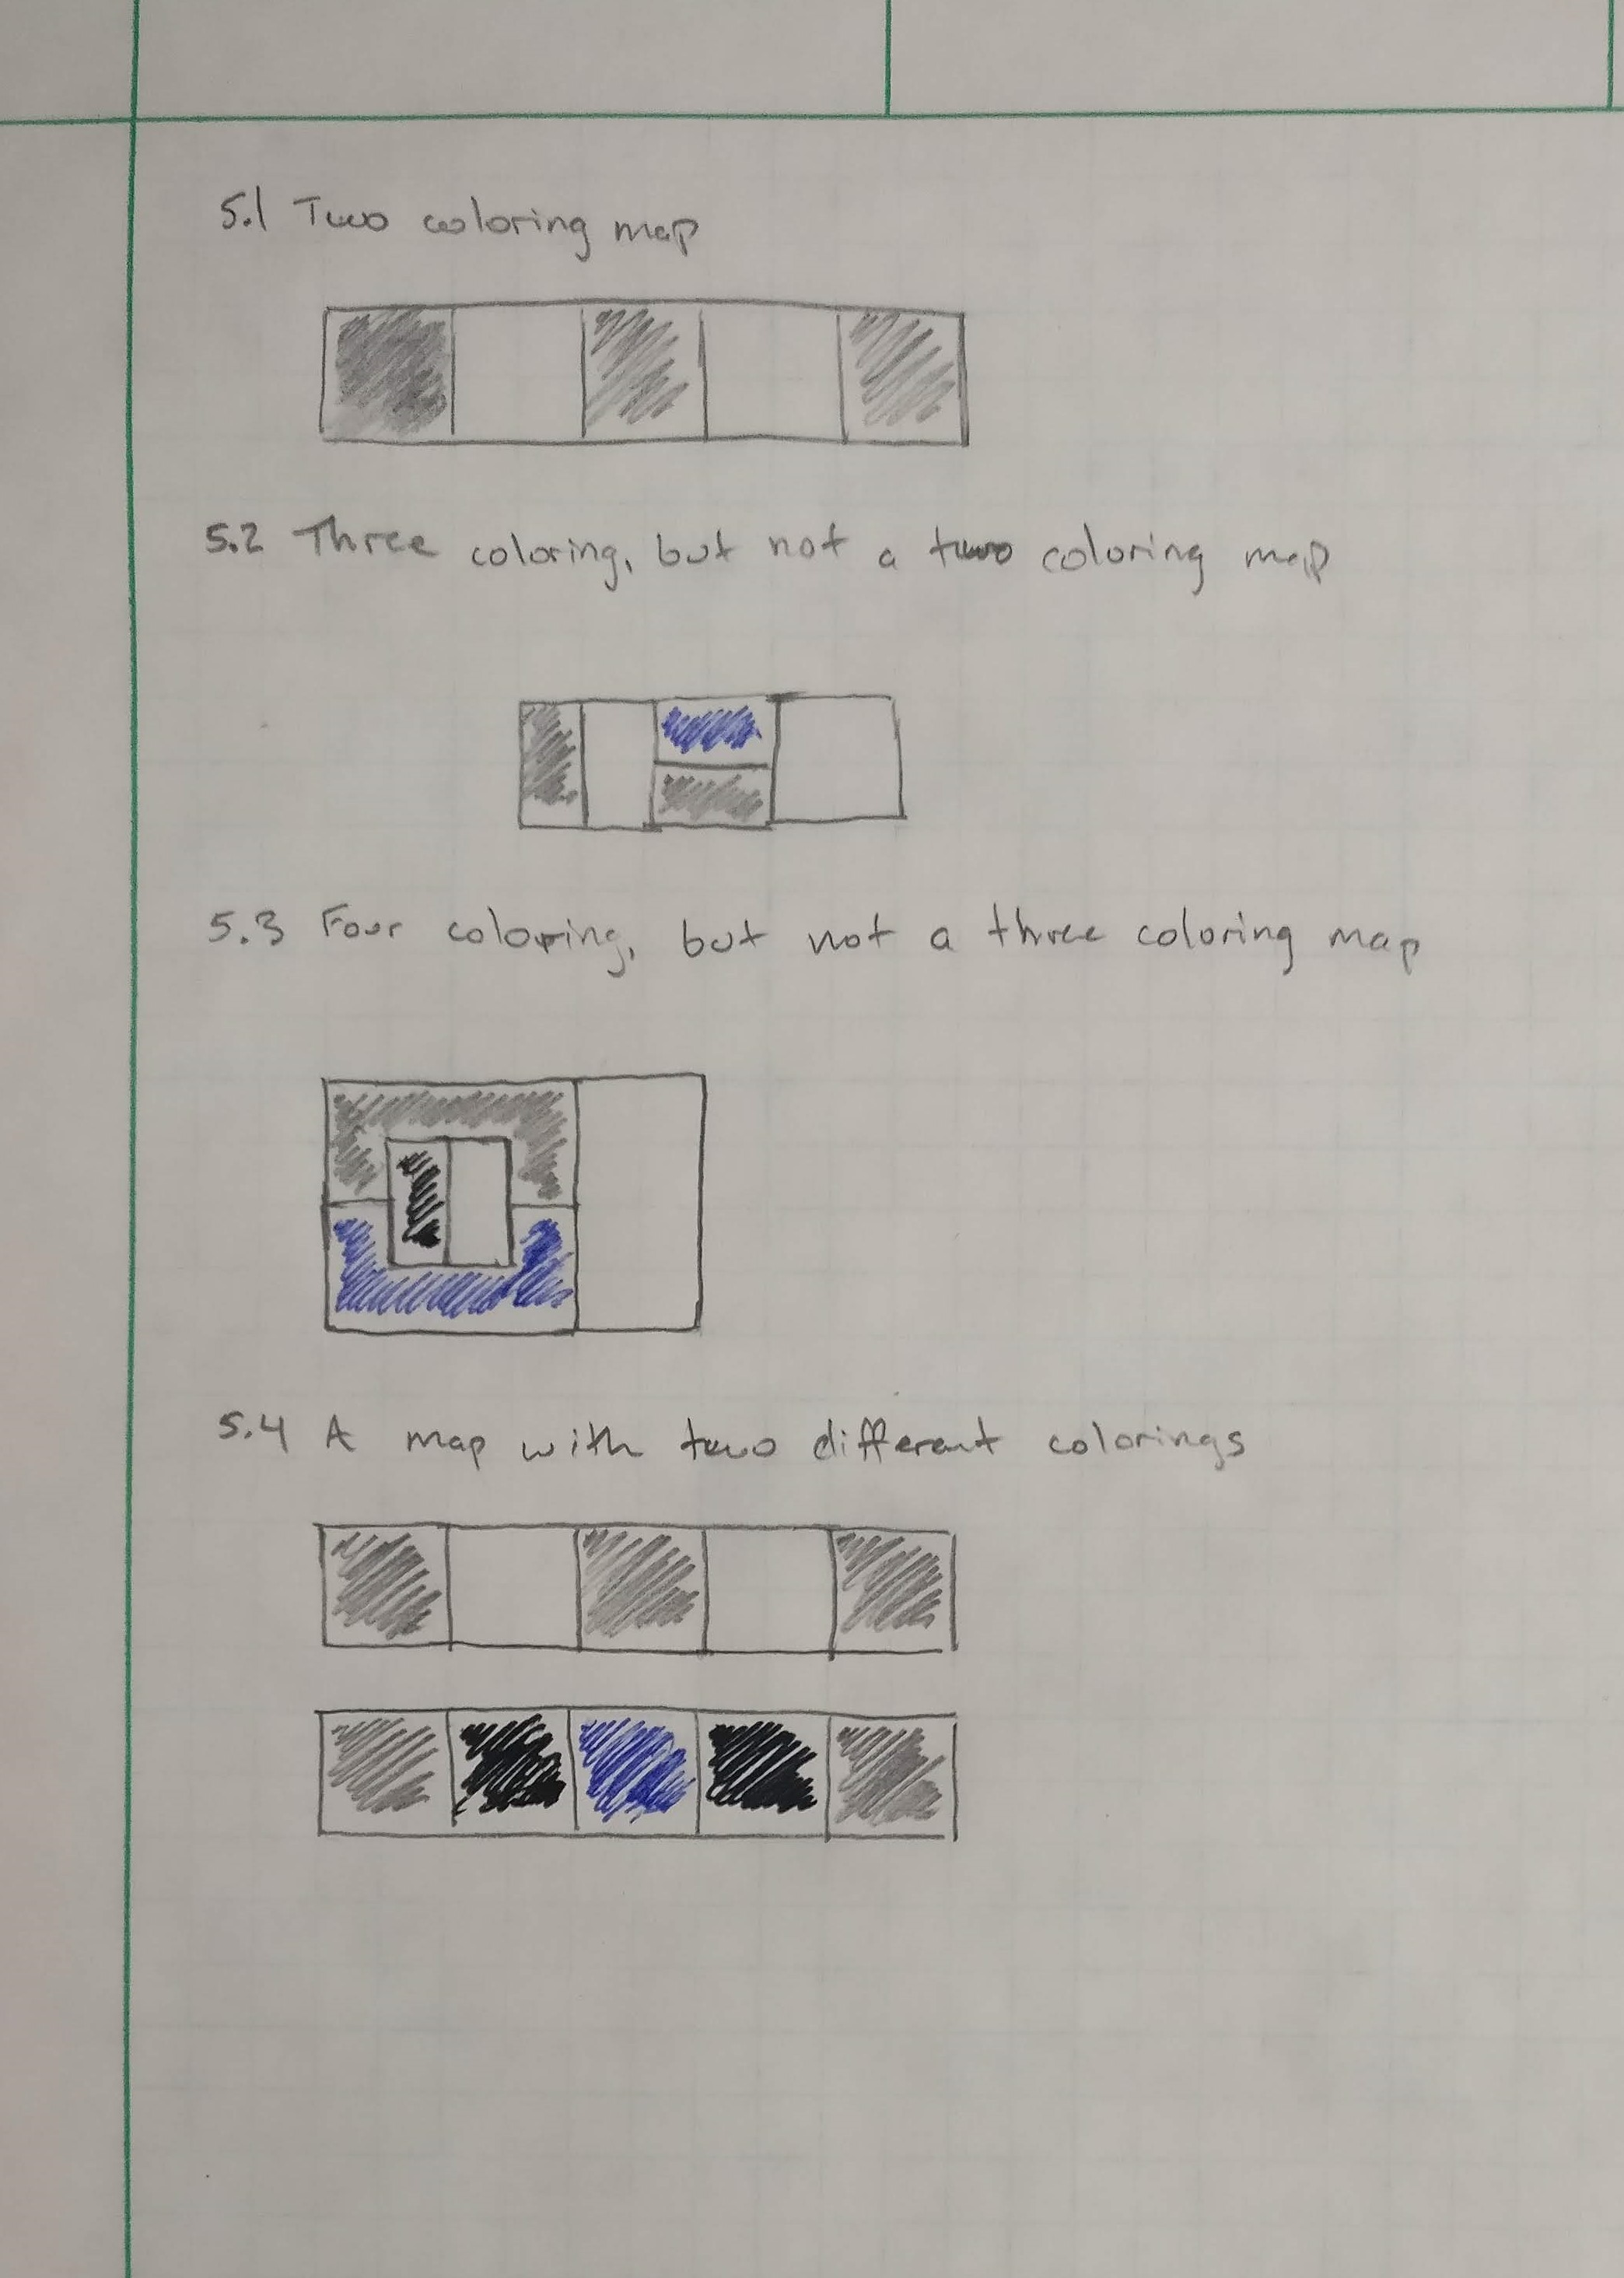
\includegraphics[width=10cm]{map_image}}
	\caption{Maps}
\end{figure}

\problem{7-6}
\collab{none}
\clearpage
\header

\section*{Leslie Gabriel Valiant}

References to online resources are provided as footnotes. \\

Leslie Valiant is an American Computer Scientist born in the mid 1950s who is famous for major contributions to artificial intelligence and parallel computing. According to the Encyclopedia Britannica, Valiant also "made key contributions to the theory of computational complexity."
\footnote{\url{https://www.britannica.com/biography/Leslie-Valiant}}
Valiant was awarded the 2010 Turing Award for his work in machine learning.

\end{document}

